%!TEX TS-program = xelatex
%!TEX encoding = UTF-8 Unicode
\documentclass[reqno ,11pt]{amsart}
\usepackage[foot]{amsaddr}
\usepackage{graphicx}
\usepackage[usenames,dvipsnames]{xcolor}
\usepackage[paperwidth=7in,paperheight=10in,text={5in,8in},left=1in,top=1in,headheight=0.25in,headsep=0.4in,footskip=0.4in]{geometry}
\usepackage{natbib}
\usepackage{subfigure}
\usepackage{lineno}
\usepackage{pdflscape}
\usepackage{afterpage}
\bibpunct[, ]{(}{)}{,}{a}{}{,}
\DeclareMathOperator{\var}{var}
\DeclareMathOperator{\cov}{cov}
\DeclareMathOperator{\E}{E}

\usepackage{tikz}
\usetikzlibrary{positioning}
\usetikzlibrary{arrows.meta}
\usepackage{extarrows} 

\synctex=1

\newcommand*\patchAmsMathEnvironmentForLineno[1]{%
  \expandafter\let\csname old#1\expandafter\endcsname\csname #1\endcsname
  \expandafter\let\csname oldend#1\expandafter\endcsname\csname end#1\endcsname
  \renewenvironment{#1}%
     {\linenomath\csname old#1\endcsname}%
     {\csname oldend#1\endcsname\endlinenomath}}% 
\newcommand*\patchBothAmsMathEnvironmentsForLineno[1]{%
  \patchAmsMathEnvironmentForLineno{#1}%
  \patchAmsMathEnvironmentForLineno{#1*}}%
\AtBeginDocument{%
\patchBothAmsMathEnvironmentsForLineno{equation}%
\patchBothAmsMathEnvironmentsForLineno{align}%
\patchBothAmsMathEnvironmentsForLineno{flalign}%
\patchBothAmsMathEnvironmentsForLineno{alignat}%
\patchBothAmsMathEnvironmentsForLineno{gather}%
\patchBothAmsMathEnvironmentsForLineno{multline}%
}

%\usepackage{lmodern}
%\usepackage{unicode-math}
\usepackage{mathspec}
\usepackage{xltxtra}
\usepackage{xunicode}
\defaultfontfeatures{Mapping=tex-text}
\setmainfont[Scale=1,Ligatures={Common}]{Adobe Caslon Pro}
\setromanfont[Scale=1,Ligatures={Common}]{Adobe Caslon Pro}
\setmathrm[Scale=1]{Adobe Caslon Pro}
\setmathfont(Digits,Latin)[Numbers={Lining,Proportional}]{Adobe Caslon Pro}

\definecolor{linenocolor}{gray}{0.6}
\definecolor{prec}{RGB}{42,115,205}
\definecolor{sens}{RGB}{255,112,0}
\definecolor{spec}{gray}{0.4}
\renewcommand\thelinenumber{\color{linenocolor}\arabic{linenumber}}

\usepackage{fix-cm}

\setcounter{totalnumber}{1}

\newcommand{\mr}{\mathrm}
\newcommand{\prim}{{\;\prime}}

\DeclareMathOperator{\dd}{d}

\renewcommand{\baselinestretch}{1.0}

\newcommand{\hatr}[2]{\mkern+#1mu \hat{\mkern-#1mu #2}}

% code for adding space to superscripts in mathmode (helps with Caslon typeface tilt)
\newcommand{\upsup}[1]{\sp{\,#1}}
\begingroup\lccode`~=`^\lowercase{\endgroup\let~\upsup}
\AtBeginDocument{%
  \catcode`^=12
  \mathcode`^="8000
}



\begin{document}

\title[Brain Structure and Vocal Repertoire]{\large Joint Inference for Brain Structure and Vocal Repertoire}
\author{Richard McElreath}
\address{Department of Human Behavior, Ecology and Culture, Max Planck Institute for Evolutionary Anthropology, Deutscher Platz 6, 04103 Leipzig, Germany}
\email{richard\_mcelreath@eva.mpg.de}
\date{\today}

%{\abstract \small x }

\maketitle

%{\vspace{-6pt}\footnotesize\begin{center}\today\end{center}\vspace{24pt}}

\linenumbers
\modulolinenumbers[5]

\section{Purpose}

Brain structure changes with age and varies by sex and population. Vocal behavior also changes with age and varies by sex and population. Under the hypothesis that brain structure influences vocal behavior, we need to estimate any causal influence of brain structure.

\subsection{Confounding expected} controlling for unobserved confounds associated with age and sex and population. For example, if brain structure and vocal behavior both are influenced by other age-related factors, then structure will be associated with vocal behavior, but the relationship may not be causal. 

\subsection{Missing data} The inference problem is made more complex by the existence of extensive missing data, imbalance, and incomplete overlap for both brain structure and vocal behavior. In the expected sample, there is extensive vocal data but much less brain structure data. The lack of complete overlap, and scarcity of data, means that attempting to mimic a classical complete case analysis would be wasteful and inefficient.

\subsection{Measurement} The primary measurements, aspects of brain connectivity and vocal repertoire, cannot be measured directly without error. 
In the case of brain connectivity, measurements are often counts that vary for reasons other than brain anatomy. The measurements must be carefully modeled to be useful in comparisons. 

In the case of vocal repertoire, the target of inference must be inferred from a finite sample, especially in the case of wild primates. This means that a strict enumeration of repertoire from observed data will usually underestimate an individual's repertoire. Since sample size differs among individuals, this problem must be dealt with statistically for comparisons to be made.

\section{Strategy}

\subsection{Concept}

We begin by specifying the heuristic causal model of the system, in order to clarify the general conditions under which a causal estimate is possible. This is also sufficient to remind us why experiments were invented.

\begin{center}
\begin{tikzpicture}
  % nodes %
  \node[text centered] (a) {$A$};
  \node[above right=1.2 of a, text centered] (b) {$B$};
  \node[below right=1.2 of a, text centered] (v) {$V$};
  \node[below right=1.2 of b, text centered] (s) {$S$};
  % edges %
  \draw[-Latex, line width= 1] (a) -- (v);
  \draw[-Latex, line width= 1] (b) -- (v);
  \draw[-Latex, line width= 1] (a) -- (b);
  \draw[-Latex, line width= 1] (s) -- (b);
  \draw[-Latex, line width= 1] (s) -- (v);
  \path[Latex-Latex,dashed] (a) edge[bend left=30] (b);
  \path[Latex-Latex,dashed] (a) edge[bend right=30] (v);
  \path[Latex-Latex,dashed] (b) edge[bend left=25] (v);
\end{tikzpicture}
\end{center}
This causal diagram includes biological effects as well as possible, but unknown, confounds of them. 
In this diagram, each letter is an observable variable: Age (A), Sex (S), Brain structure (B), and Vocal behavior (V). The arrows represent causal relationships. The dashed paths represent plausible unobserved confounds of unknown strength.

%[how to discuss age-period-cohort problem?]
The unobserved confounds connecting $A$ to $B$ and $V$ represent unknown period and cohort effects that mimic age but are causally unrelated to biological aging. In principle any association with age could be explained in part by period (year specific events) and cohort (interaction between period and age) effects. We don't try to resolve this unresolvable problem. But we do exercise caution in interpreting associations with age.


\subsection{Causal inference}

To merely describe the age-related association between brain structure and vocal behavior, we can measure the association while stratifying by age (and sex if needed). However, to interpret these associations as causal requires a lot more. Our goal is to be transparent about the assumptions that are biologically plausible and which sorts of inference they justify.

Using the previous DAG and knowledge of d-separation and the backdoor criterion of do-calculus, we can derive the general conditions under which inference of the causal effect of $B$ on $V$ is possible, $p(V|\mathrm{do}(B))$.
First notice that there are backdoor paths through $A$ and $S$. Stratification by $A$ and $S$ is sufficient to block these paths. So we must stratify by age and sex in order to estimate $B \rightarrow V$. 

The unobserved confounds connecting $A$ to $B$ and $V$ represent unknown period and cohort effects that mimic age but are unrelated to biological aging. These paths are problematic. If we stratify by age, then age becomes a collider on $B \longleftrightarrow A \longleftrightarrow V$. Therefore it is not possible to control for unknown cohort effects.

The unobserved confound connecting $B$ and $V$ obviously causes problems. This could arise from factors like common family exposure that is unobserved but generates association between brain structure and vocal behavior across families. It is impossible to exclude the possibility of unobserved confounds, but it is possible to calculate how strong the confounds must be to remove any apparently causal effect of $B$ on $V$.

In summary, while it is not possible in theory to eliminate all plausible confounding, it is possible to interpret estimates correctly as mixes of causal and confound effects. For example, if we are willing to assume that cohort effects and unobserved confounds between $B$ and $V$ are absent, then stratification by $A$ and $S$ is sufficient to estimate the causal influence of $B$ on $V$. Any estimated coefficient in such an analysis will likely be an upper bound, due to unobserved cohort or other confounds.

\subsection{Missing data}

When some data are missing, we must augment the causal model to simultaneously model to missingness mechanism. The cause of missing values tells us whether they are ignorable or rather how to impute them.

Consider the example below, in which the previous causal diagram is augmented with missingness nodes $R$ that point into observed variables with stars $\star$ that indicate variables containing missing values. The corresponding variable without the $\star$ is unobserved (no missing values). 

\begin{center}
  \begin{tikzpicture}
    % nodes %
    \node[text centered] (a) {$A$};
    \node[above right=1.2 of a, text centered] (b) {$B$};
    \node[below right=1.2 of a, text centered] (v) {$V$};
    \node[below right=1.2 of b, text centered] (s) {$S$};
    \node[left=1.0 of b, text centered] (bo) {$B\star$};
    \node[left=1.0 of bo, text centered] (Rb) {$R_B$};
    \node[left=1.0 of v, text centered] (vo) {$V\star$};
    \node[left=1.0 of vo, text centered] (Rv) {$R_V$};
    % edges %
    \draw[-Latex, line width= 1] (a) -- (v);
    \draw[-Latex, line width= 1] (b) -- (v);
    \draw[-Latex, line width= 1] (a) -- (b);
    \draw[-Latex, line width= 1] (s) -- (b);
    \draw[-Latex, line width= 1] (s) -- (v);
    \path[Latex-Latex,dashed] (a) edge[bend left=30] (b);
    \path[Latex-Latex,dashed] (a) edge[bend right=30] (v);
    \path[Latex-Latex,dashed] (b) edge[bend left=25] (v);
    \draw[-Latex, line width= 1] (Rb) -- (bo);
    \draw[-Latex, line width= 1] (b) -- (bo);
    \draw[-Latex, line width= 1] (a) -- (Rb);
    \draw[-Latex, line width= 1] (v) -- (vo);
    \draw[-Latex, line width= 1] (Rv) -- (vo);
  \end{tikzpicture}
  \end{center}

Consider $V$ first. In this example, we observe only $V\star$, which is influenced by the true values $V$ and the missingness mechanism $R_V$. This is the most benign form of missing data, \emph{missing completely at random}. The association between $B$ and $V$ cannot be confounded by the missingness. It is only harder to measure. The causal model can be used to impute missing values, so that incomplete cases do not need to be dropped. But this is not strictly necessary for valid inference.

Now consider instead $B$. In this case, the missingness mechanism $R_B$ is itself influenced by another variable, age ($A$). This is very plausible, since individuals of some ages are more likely to die and therefore contribute brain samples. In this case, there is a backdoor path through $A$ that confounds inference of $B \rightarrow V$. We must condition of $A$ to close that path, blocking the influence of $R_B$. 

As explained before, if there are unobserved cohort effects (the dashed paths between $B$, $A$ and $V$) then conditioning on $A$ will introduce a new confound that cannot be adjusted for. But that situation is not new. It is not caused by the missing $B$ values.

So what can we do? For each variable with missing values, we must state what influences missingness. If missingness is caused by an observed variable (like $A$), usually we can adjust for it and proceed as before. We can impute missing values as well, to retain as much efficiency in estimation as possible. 

But if any pattern of missingness is caused by the variable itself, then we must model the missingness mechanism or otherwise give up. For example, in censored time-to-event data the values that are missing are missing exactly because of their value: the event happened after the sampling period ended. These missing values cannot be ignored. And no other observed variable can be conditioned on to resolve the problem. So instead we model the censoring process and use it to impute the missing values. That is indeed the standard justification for time-to-event analysis, where censored observations must be included in the analysis but modeled differently than observed values.


\subsection{Measurement error}

For both $B$ and $V$, we expect only imperfect estimates. We can augment our causal diagram with observed variables $B^\circ$ and $V^\circ$, similar to how we added $B\star$ and $V\star$. The key assumption is that only observed variables influence measurement error, and that we can model their influence.


\subsection{Reciprocal causation}

An alternative causal model posits a feedback between brain structure and vocal behavior over time. In this case, any association between brain structure and vocal behavior cannot be interpreted as the influence of one on the other. Without a time series of brain and vocal measurements, it is not possible to do more. 
However, it is possible to specify a generative model, using for example ODEs, to express the hypothesis. 



\subsection{Vocal variables}

The variables that stand for vocal behavior must be inferred from individual recordings. Individual chimpanzees are represented by different numbers of recordings. In many cases there are hundreds of recordings. But other individuals have only 1 recording. 

We focus on the example of \emph{vocal repertoire}, the number of distinct vocalizations in an individuals behavior repertoire. 
[repertoire text]


\subsection{Brain structure variables}
x


\section{Implementation}

We implement a complete generative model, corresponding to the heuristic causal model, so that we can produce synthetic data that allows us to (1) clarify the hypothetical relationships among variables (through forward simulation) and (2) validate the statistical implementation (through inverse inference).

\subsection{Structural relationships}

The core structural model connects observed and inferred variables. Let $\star$ indicate the observed measurement. For example, $B\star$ is a brain measurement, and $B$ is the inferred structural trait. Then:
\begin{align*}
  B_i &\sim f_1 ( A_i , S_i )\\
  V_i &\sim f_2 ( B_i , A_i , S_i  )\\
  B_i^\star &\sim f_3 ( B_i )\\
  V_i^\star &\sim f_4 ( V_i )
\end{align*}
The functions $f_1$ and $f_2$ model the causal relationships among the variables. The functions $f_3$ and $f_4$ model the measurement process. Age $A_i$ could be added to the measurement functions, if for example measurement error depends upon age.

\subsection{Functional relationships}

To go beyond the structural relationships towards estimation, we need to make assumptions about how variables relate causally, not just whether or not they do. This applies to both the measurement models and the inferential models.

\subsubsection{Brains}
Let's begin with the brain structure measurements, $B$. The first problem is that the true brain structure is measured with error.
[description of measurement process here---science magic!] 
This leads us to model the observed structural measure, $B^\star$, as an over-dispersed Poisson variable with a known offset $b_i$ for each measurement.
\begin{align*}
  B_i^\star &\sim \text{gamma-Poisson} ( \mu_i , \tau ) \\
  \mu_i &=  B_i^\theta  \times b_i
\end{align*}

The $B$ parameters are then used to model the relationship between age and brain structure. There are many functional choices here, but the most basic is perhaps a simple sigmoid, which serves to illustrate the concept.
\begin{align*}
  B_i &= \text{logit}^{-1} \big( \beta_{S[i]}(A_i - \alpha) + z_i \big)\\
  z_i &\sim \text{normal}(0,1)
\end{align*}
where $A_i$ is the age of the specimen, $\alpha$ determines the inflection point in brain development, $\beta$ is a sex-specific rate parameter, and $z_i$ is an individual residual from the developmental norm.

\subsubsection{Vocalization} 

The first vocalization measure we address is \emph{vocal repertoire}, the total number of unique vocalizations an individual can produce. In principle, an individual's repertoire can be estimated by simply counting the number of unique vocalizations they have been heard to produce. However this naive estimate will be biased downwards from the true repertoire, because any finite sample may miss some vocalizations. In a very small sample, even vocalizations that are often produced could be missed. The relationship between the bias and sample size is complex, depending upon the rates of production of different vocalizations, as well as how common each is. We address this by modeling the sampling process and estimating the unobserved true repertoire as a latent variable. 

Suppose a population of $N$ individuals (monkeys, people) who produce among them $M$ different vocalizations. Each individual has potentially a different repertoire of these $M$ vocalizations. We seek a vector $\phi$ of posterior probability distributions of length $M$ for each individual $i$. In the case that $i$ was observed to produce a $m$, then $\phi_m$ is 1. But when $m$ was not observed, we can compute the posterior probability that this was due to the finite sample, an undercount. 
In the simplest model, assume that each vocalization $m$ is produced at a rate $\lambda_m$, when an individual possesses it. This produces a Poisson distribution of the counts $Y_{i,j,m}$ of each possessed vocalization $m$ in a focal recording $j$ of duration $d_j$.
\begin{align*}
Y_{i,j,m} &\sim \mathrm{Poisson}(  \lambda_m \, d_j \, x_{i,m} )
\end{align*}
where $x_{i,m}$ is an indicator variable for whether individual $i$ possesses vocalization $m$. 
When the observed $y=Y_{i,j,m}>0$, then the probability is:
\begin{align*}
\Pr(y|y>0) &= p_{m} \frac{( \lambda_m d_j )^y \exp(-\lambda_m d_j) }{ y! }
\end{align*}
where $p_m$ is the probability an individual possesses $m$. When $y=0$ is observed, we require a mixture:
\begin{align*}
\Pr(y|y=0) &= p_{m} \exp(-\lambda_m d_j) + (1-p_{m})(1)
\end{align*}

If the estimated repertoire of an individual is of interest, these can be calculated post-sampling. Let $X_{i,m}$ be the total number of times $i$ was observed to use $m$ and $D_{i}$ be the total sampling effort (duration of recordings). If $X_{i,m}>0$, then $i$ possesses the vocalization. But what about when $X_{i,m}=0$? In that case, the posterior probability that individual $i$ possesses vocalization $m$ follows from Bayes' rule:
\begin{align*}
	\Pr(x_{i,m}=1|X_{i,m}=0,D_{i}) &= \frac{\Pr(0|x_{i,m}=1)\Pr(x_{i,m}=1)}{\Pr(0)} \\ 
	&= \frac{\Pr(0|\lambda_m D_{i})p_m}{\Pr(0|\lambda_m D_{i})p_m + (1-p_m)}
\end{align*}
And this is sufficient to compute the posterior probability that each vocalization is in the repertoire, the vector $\phi$.

The individual repertoires are not needed however for inference about associations between age, brain structure, and elements of the repertoire. 
To model the relationship between repertoire and development, we want to introduce functional relationships with age and brain structure, possibly stratified by sex. 
As an example of extending the model, we can modify the probabilities $p$ so they are an increasing function of individual age. This implies that older individuals possess on average more unique vocalizations. A simple model says that the probability an individual of age $A$ possesses vocalization $m$ is:
\begin{align*}
	p_m(A) = \alpha_m ( 1 - \exp(-\beta_m A) ) ^{\gamma_m}
\end{align*}
where $\alpha_m$ is the maximum probability for $m$, $\beta_m$ is the rate of increase with age, and $\gamma_m$ is the ``elasticity'' with age (which allows for slow initial increases when $\gamma_m > 1$).

The above is the total effect of age on repertoire, but some of this relationship is due to brain structure. A simple approach is to adopt a symmetric relationship for both age and brain structure:
\begin{align*}
	p_m(A) = \alpha_m ( 1 - \exp(-\beta_{Am} A)\exp(-\beta_{Bm} B) ) ^{\gamma_m}
\end{align*}
This allows both age and brain structure to contribute to the probability of inclusion in the repertoire. But both count towards the same asymptote, $\alpha_m$.

A similar construction allows stratification of rates of production by age and brain structure:
\begin{align*}
	\lambda_m(A,B) = L_m ( 1 - \exp(-\beta_{Am} A)\exp(-\beta_{Bm} B) ) ^{\gamma_m}
\end{align*}


\section{Statistical model and estimation algorithm}

The generative model above can be specified directly as a statistical model. Any probabilistic programming language is sufficient. We use Stan (mc-stan.org), because of its flexibility, advanced sampling algorithms, and portability across scripting languages.

\subsection{Data model}
x

\subsection{Priors}
x

\subsection{Prior predictive simulations}
x

\subsection{Bayesian imputation}

Bayesian imputation of missing values is straightforward for continuous variables. For discrete variables, like a Poisson count, the code will need to marginalize over unknowns. Such code can be slow, but given that the sample size is rather small, this is not an obstacle yet.

\section{Validation}

x

\begin{verbatim}
       mean   sd  5.5% 94.5% rhat ess_bulk
bA     0.13 0.01  0.11  0.16 1.00  1368.82
bB     0.91 0.29  0.47  1.41 1.00  1711.20
delta  1.01 1.09  0.06  2.87 1.00  1832.18
alpha  7.00 0.29  6.54  7.43 1.00   586.13
tau   22.93 3.87 17.17 29.43 1.00  1563.79
theta  0.77 0.13  0.59  1.01 1.00   484.59
bXV    0.00 0.52 -0.79  0.83 1.00  3089.47
bXB    0.01 0.51 -0.82  0.84 1.01  3906.02
\end{verbatim}

\begin{center}
	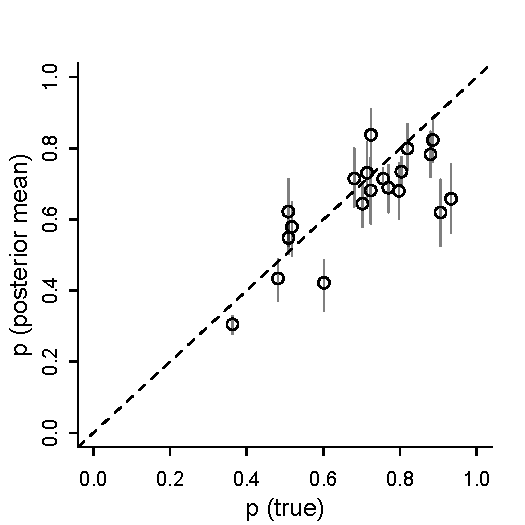
\includegraphics[scale=0.7]{fig_validate_p.pdf}~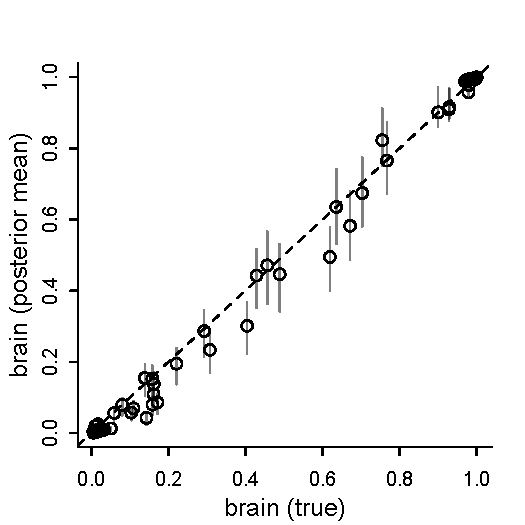
\includegraphics[scale=0.7]{fig_validate_brain.pdf}
\end{center}

%%%%%%%%%%%%%%%%%%%%%%%
\clearpage
\bibliographystyle{apalike} 
\bibliography{references}

\end{document}








